\documentclass[border=5mm]{standalone}
\usepackage{tikz}
\usepackage{amsmath, amssymb}\usetikzlibrary{positioning}
\usepackage{graphicx}
\usetikzlibrary{positioning,calc,arrows.meta,shapes.geometric}

\begin{document}
% Coordinate map: the cell-state highway runs from C_{t-1} at upper left to
% C_t at upper right; h_{t-1} and x_t feed four gates down the left; the
% candidate and retained state meet at +; the lower-right branch produces h_t.
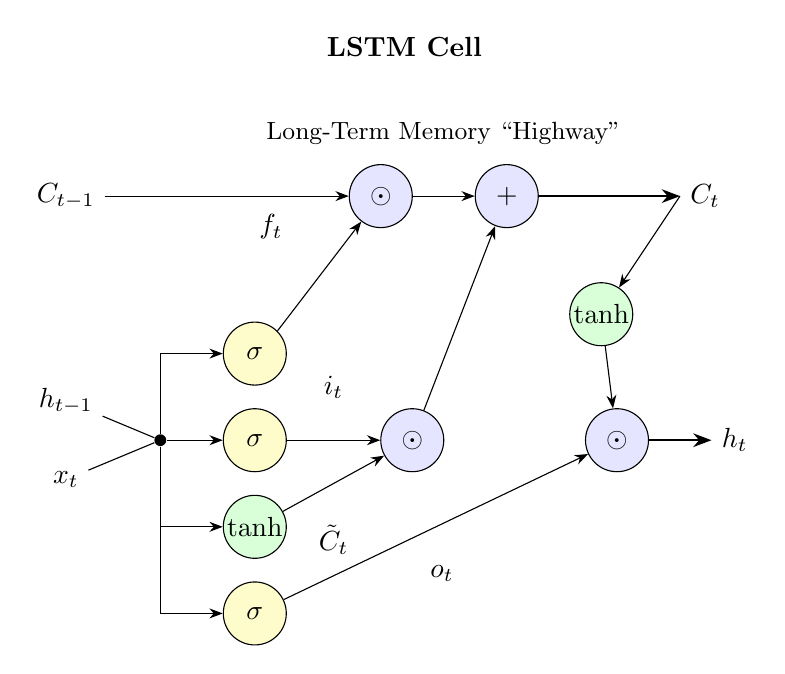
\begin{tikzpicture}[
  >=Stealth,
  node distance=0.9cm and 1.2cm,
  gate/.style={circle, draw, fill=yellow!20, minimum size=8mm, inner sep=0pt},
  tanh/.style={circle, draw, fill=green!15, minimum size=8mm, inner sep=0pt},
  op/.style={circle, draw, fill=blue!10, minimum size=8mm, inner sep=0pt},
  cell/.style={draw, rounded corners, thick, inner sep=8mm}
]

% Bounding box of the LSTM cell
%\node[cell, minimum width=9.8cm, minimum height=6.2cm] (cellbox) at (3.5,0) {};

% Inputs (left)
\node (hprev) at (-0.8,-1.6) {$h_{t-1}$};
\node (xt)    at (-0.8,-2.6) {$x_t$};
\node (cprev) at (-0.8,  1.0) {$C_{t-1}$};


% Junction for h_{t-1}, x_t
\node[circle, fill=black, inner sep=0pt, minimum size=1.5mm] (split) at (0.4,-2.1) {};
\draw (hprev) -- (split);
\draw (xt)    -- (split);

% Gates and nonlinearity inputs
\node[gate] (f) at (1.6,-1.0) {$\sigma$};
\node[gate] (i) at (1.6,-2.1) {$\sigma$};
\node[tanh] (g) at (1.6,-3.2) {$\tanh$};
\node[gate] (o) at (1.6,-4.3) {$\sigma$};

% Wire split to gates
\draw[->] (split) |- (f);
\draw[->] (split) -- (i);
\draw[->] (split) |- (g);
\draw[->] (split) |- (o);

% Forget path: C_{t-1} --x f_t
\node[op] (times_f) at (3.2,1.0) {$\odot$};
\draw[->] (cprev) -- (times_f);
\draw[->] (f.north east) -- node[pos=0.46, above left=4mm and 3mm] {$f_t$} (times_f);

% Input path: i_t x \tilde{C}_t
\node[op] (times_i) at (3.6,-2.1) {$\odot$};
\draw[->] (i) -- node[pos=0.5, above=4mm] {$i_t$} (times_i);
\draw[->] (g) -- node[pos=0.5, below=4mm] {$\tilde{C}_t$} (times_i);

% Cell state add
\node[op] (plus) at (4.8,1.0) {$+$};
\draw[->] (times_f) -- (plus);
\draw[->] (times_i) -- (plus);

% Cell state output C_t and highway
\coordinate (ct) at (7.0,1.0);
\draw[->,thick] (plus) -- (ct) node[right] {$C_t$};

% Highway label
\node at (4,1.8) {\small Long-Term Memory ``Highway''};

% Output path: tanh(C_t) × o_t -> h_t
\node[tanh] (tanh_ct) at (6.0,-0.5) {$\tanh$};
\node[op]   (times_o) at (6.2,-2.1) {$\odot$};

\draw[->] (ct) -- (tanh_ct);
\draw[->] (tanh_ct) -- (times_o);
\draw[->] (o) -- node[pos=0.52, below=4mm] {$o_t$} (times_o);

\coordinate (hout) at (7.4,-2.1);
\draw[->,thick] (times_o) -- (hout) node[right] {$h_t$};

% Title inside cell
\node at (3.5,2.9) {\bfseries LSTM Cell};

\end{tikzpicture}\end{document}
